\documentclass[11pt]{beamer}

% Theme and packages
\usetheme{Madrid}
\usecolortheme{default}
\usepackage{amsmath, amssymb, amsfonts}
\usepackage{tikz}
\usetikzlibrary{shapes.geometric, arrows}

% Flowchart styles
\tikzstyle{startstop} = [rectangle, rounded corners, minimum width=3cm, minimum height=1cm,text centered, draw=black, fill=red!30]
\tikzstyle{process} = [rectangle, minimum width=3cm, minimum height=1cm, text centered, draw=black, fill=blue!20]
\tikzstyle{decision} = [diamond, aspect=2, text centered, minimum width=3cm, draw=black, fill=green!20]
\tikzstyle{arrow} = [thick,->,>=stealth]

% Title information
\title[Factorization of Ideals]{Factorization of Algebraic Ideals and Its Applications}
\author{Your Name}
\institute{Your Affiliation}
\date{\today}

\begin{document}

%----------------------------------
% Title Slide
%----------------------------------
\begin{frame}
  \titlepage
\end{frame}

%----------------------------------
\begin{frame}{Motivation}
\begin{itemize}
  \item Ideal decomposition simplifies systems of polynomial equations.
  \item Provides structure for algebraic and geometric analysis.
  \item Fundamental tool for both theory and computation.
\end{itemize}
\end{frame}

%----------------------------------
\begin{frame}{Background: Ideals in Commutative Algebra}
\begin{columns}
\column{0.55\textwidth}
\begin{itemize}
  \item An \textbf{ideal} $I \subset R$ is a subset closed under addition and multiplication by ring elements.
  \item \textbf{Prime ideal:} if $ab \in P$, then $a \in P$ or $b \in P$.
  \item \textbf{Primary ideal:} if $ab \in Q$, then $a \in Q$ or $b^n \in Q$.
\end{itemize}
\column{0.45\textwidth}
\centering
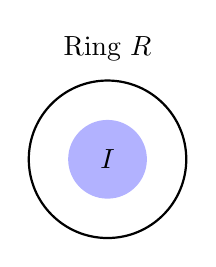
\begin{tikzpicture}
  \draw[thick] (0,0) circle (1);
  \node at (0,1.4) {Ring $R$};
  \fill[blue!30] (0,0) circle (0.5);
  \node at (0,0) {$I$};
\end{tikzpicture}
\end{columns}
\end{frame}

%----------------------------------
\begin{frame}{Prime and Primary Decomposition}
\begin{columns}
\column{0.55\textwidth}
\begin{itemize}
  \item Decomposing an ideal as an intersection of prime ideals.
  \item Geometric viewpoint: corresponds to union of algebraic varieties.
  \item Analogy with integer factorization.
\end{itemize}
\column{0.45\textwidth}
\centering
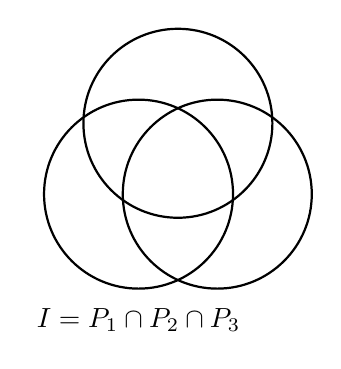
\begin{tikzpicture}
  \draw[thick] (0,0) circle (1.2);
  \draw[thick] (1,0) circle (1.2);
  \draw[thick] (0.5,0.9) circle (1.2);
  \node at (0, -1.6) {$I = P_1 \cap P_2 \cap P_3$};
\end{tikzpicture}
\end{columns}
\end{frame}

%----------------------------------
\begin{frame}{Classical Results}
\begin{itemize}
  \item \textbf{Lasker–Noether theorem}: Every ideal in a Noetherian ring admits a primary decomposition.
  \item Uniqueness up to radicals and associated primes.
\end{itemize}
\end{frame}

%----------------------------------
\begin{frame}{Algorithms for Ideal Factorization}
\centering
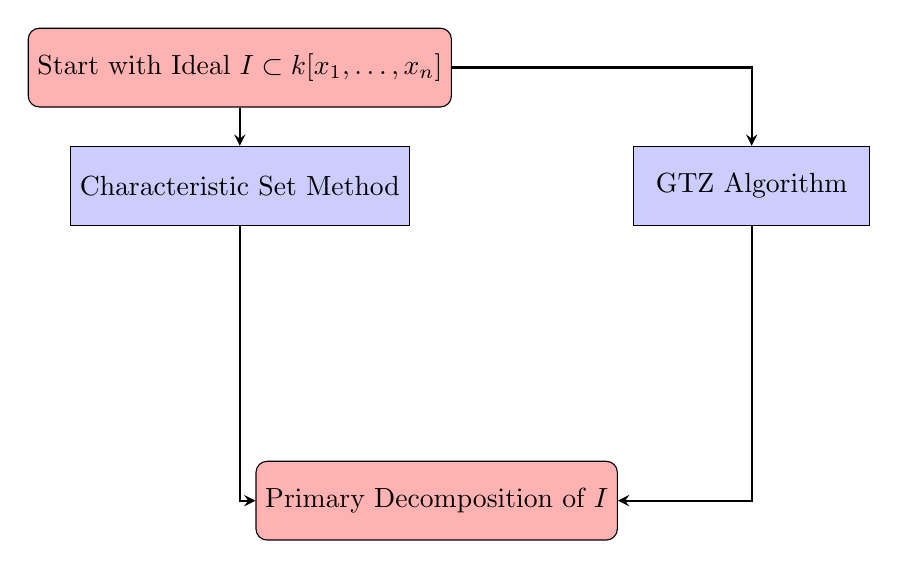
\begin{tikzpicture}[node distance=1.5cm]
\node (start) [startstop] {Start with Ideal $I \subset k[x_1,\dots,x_n]$};
\node (cs) [process, below of=start] {Characteristic Set Method};
\node (gtz) [process, right of=cs, xshift=5cm] {GTZ Algorithm};
\node (end) [startstop, below of=cs, yshift=-2.5cm, xshift=2.5cm] {Primary Decomposition of $I$};

\draw [arrow] (start) -- (cs);
\draw [arrow] (start) -| (gtz);
\draw [arrow] (cs) |- (end);
\draw [arrow] (gtz) |- (end);
\end{tikzpicture}
\end{frame}

%----------------------------------
\begin{frame}{Characteristic Set Method}
\begin{itemize}
  \item Uses elimination and triangular sets.
  \item Originates in differential algebra.
  \item Advantage: systematic structure.
  \item Limitation: ordering choice is crucial.
\end{itemize}
\end{frame}

%----------------------------------
\begin{frame}{GTZ Algorithm}
\begin{itemize}
  \item Gröbner basis-based.
  \item Splits and refines components iteratively.
  \item Widely implemented in CAS.
\end{itemize}
\centering
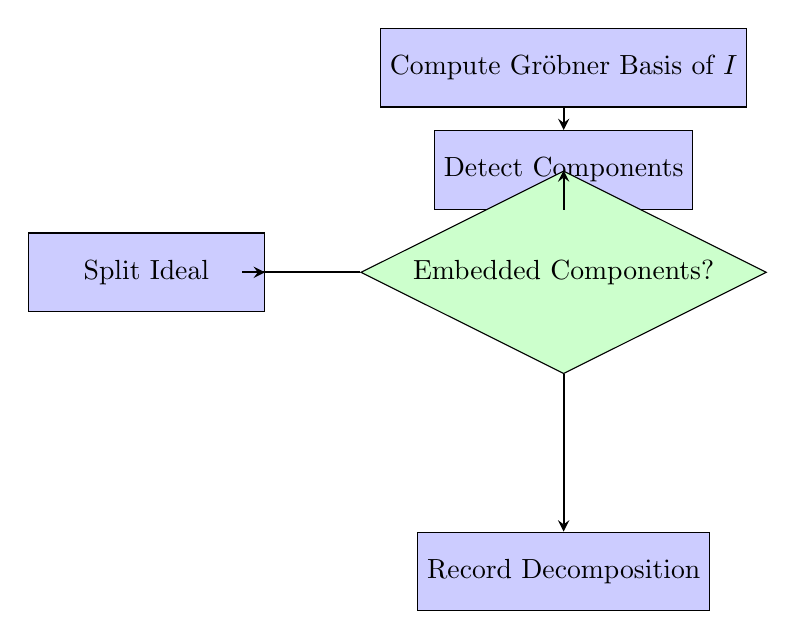
\begin{tikzpicture}[node distance=1.3cm]
\node (gb) [process] {Compute Gröbner Basis of $I$};
\node (comp) [process, below of=gb] {Detect Components};
\node (split) [decision, below of=comp] {Embedded Components?};
\node (splityes) [process, left of=split, xshift=-4cm] {Split Ideal};
\node (no) [process, below of=split, yshift=-2.5cm] {Record Decomposition};

\draw [arrow] (gb) -- (comp);
\draw [arrow] (comp) -- (split);
\draw [arrow] (split.west) -- ++(-1.5,0) -- (splityes.east);
\draw [arrow] (split.south) -- ++(0,-1) -- (no.north);
\end{tikzpicture}
\end{frame}

%----------------------------------
\begin{frame}{Worked Example 1}
\begin{itemize}
  \item Example: $I = \langle x^2-y, \, xy \rangle \subset k[x,y]$
  \item Gröbner basis computation $\rightarrow$ decomposition.
  \item Interpreted geometrically as simpler varieties.
\end{itemize}
\centering
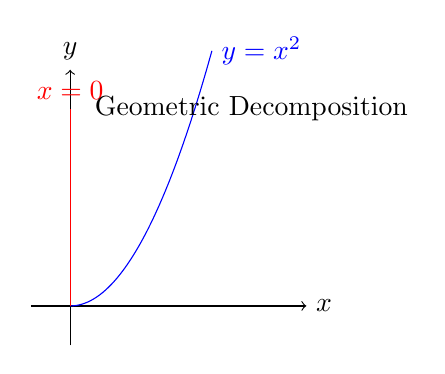
\begin{tikzpicture}
  \draw[->] (-0.5,0) -- (3,0) node[right] {$x$};
  \draw[->] (0,-0.5) -- (0,3) node[above] {$y$};
  \draw[domain=0:1.8,smooth,variable=\x,blue] plot ({\x},{\x*\x}) node[right] {$y=x^2$};
  \draw[red] (0,0) -- (0,2.5) node[above] {$x=0$};
  \node at (2.3,2.5) {Geometric Decomposition};
\end{tikzpicture}
\end{frame}

%----------------------------------
\begin{frame}{Applications to Polynomial Equations}
\begin{itemize}
  \item Decomposition $\Leftrightarrow$ splitting solution sets.
  \item Ideal $\cap$ decomposition $\Rightarrow$ variety union.
\end{itemize}
\centering
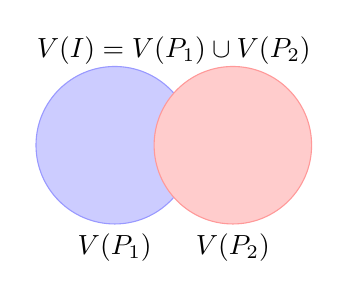
\begin{tikzpicture}
  \draw[blue!40,fill=blue!20] (0,0) circle(1);
  \draw[red!40,fill=red!20] (1.5,0) circle(1);
  \node at (0,-1.3) {$V(P_1)$};
  \node at (1.5,-1.3) {$V(P_2)$};
  \node at (0.75,1.2) {$V(I)=V(P_1)\cup V(P_2)$};
\end{tikzpicture}
\end{frame}

%----------------------------------
\begin{frame}{Applications to Differential Equations}
\begin{itemize}
  \item Characteristic set methods connect differential systems with ideals.
  \item Decomposition splits families of solutions.
\end{itemize}
\end{frame}

%----------------------------------
\begin{frame}{Current Limits and Open Problems}
\begin{itemize}
  \item Complexity is often exponential.
  \item Gröbner basis can be costly.
  \item Future directions:
    \begin{itemize}
      \item Hybrid and numerical-symbolic methods.
      \item Parallelization.
    \end{itemize}
\end{itemize}
\end{frame}

%----------------------------------
\begin{frame}{Summary and Conclusions}
\begin{itemize}
  \item Every ideal in a Noetherian ring can be decomposed.
  \item Algorithms (Characteristic Set, GTZ) make this practical.
  \item Applications: polynomial and differential systems.
\end{itemize}
\end{frame}

%----------------------------------
\begin{frame}{Questions?}
  \centering
  \Huge Thank you! \\
  \vspace{1cm}
  \Large Questions welcome.
\end{frame}

\end{document}
